\documentclass[a4paper]{article}
\usepackage[margin = 1 in]{geometry}
\usepackage{fancyhdr}
\usepackage{lastpage}
\usepackage{ctex}
\usepackage[utf8]{inputenc} % Required for inputting international characters
\usepackage[T1]{fontenc} % Output font encoding for international characters
\usepackage[sfdefault]{ClearSans} % Use the Clear Sans font (sans serif)
\usepackage{tocloft} 
\usepackage{makecell}%导入表格宏包
\usepackage{bmpsize}
\usepackage{graphicx}
\usepackage{epstopdf}
\usepackage{caption}
\usepackage{enumitem}
\usepackage{float}
\usepackage{multirow}
\usepackage{makecell}
\usepackage{wrapfig}
\usepackage{tcolorbox}
\usepackage[hidelinks]{hyperref}
\usepackage{xcolor}

\pagestyle{fancy}
\lhead{\textsl{\href{https://13.40.143.199/}{\textcolor{blue}{Team Project}}}}
\chead{}
\rhead{Page \thepage\ of \pageref{LastPage}}
\lfoot{}
\rfoot{}
\cfoot{}
\renewcommand{\headrulewidth}{0.4pt}
\renewcommand{\footrulewidth}{0pt}
\renewcommand{\cftsecleader}{\cftdotfill{\cftdotsep}}
\newcommand{\tabincell}[2]{\begin{tabular}{@{}#1@{}}#2\end{tabular}} %单元格内换行

\renewcommand*\contentsname{Table of Contents}

\begin{document}

%----------------------------------------------------------------------------------------
%	TITLE PAGE
%----------------------------------------------------------------------------------------

\begin{titlepage}
	
	\rule{\linewidth}{5pt}
	\raggedleft
	\fontsize{38pt}{50pt}\selectfont
    \textbf{\\Team Project\\}
    \fontsize{28pt}{60pt}\selectfont 
    for\\
    \fontsize{38pt}{60pt}\selectfont 
    \textbf{Milestone 2\\}
	
	\vfill % Space between the title box and author information
	
	%------------------------------------------------
	%	Author name and information
	%------------------------------------------------
	
	\parbox[t]{0.93\textwidth}{ % Box to inset this section slightly
		\raggedleft % Right align the text
		\large % Increase the font size
		{\Large By Team 23-22}\\[4pt] % Extra space after name
		Bogdan-Marian Gheorghe\_2329324\_bxg125\\
		Chance Egbon\_2194210\_cee010\\
		Gilead Bempah\_2296232\_gxb035\\
		Matthew Goulding\_2330080\_mxg183\\
		Samuel Okasia\_2345883\_sxo183\\
		Smit Navinkumar\_2327596\_sxn197\\
		Zijun Li\_2272583\_zxl183\\
	}
	
\end{titlepage}

\begin{center}
	\tableofcontents
	\addcontentsline{toc}{section}{Table of Contents}
\end{center}
\newpage

\section{S2 ranking}

{\noindent\begin{tabular}{|p{0.075\linewidth}|p{0.25\linewidth}|p{0.55\linewidth}|} 
	\hline
 \textbf{Rank} & \textbf{Name} & \textbf{Comments} \\
 \hline
 1 & Zijun Li & The To-Do List feature allows the user to create new task providing useful information such as a Heading, and description while also providing the user with a visual  representation of the tasks sorted as to-dos and Dones. The tasks will also be sorted by priority and will work together with the scheduler and the Notification system to improve the user's awareness. The technical report provides a good explanation about what an API is and how it works, while also presenting the benefits and drawbacks that could occur. Also the report provides reasoning for using APIs in the time management application while also providing some common use cases where an API would be needed. \\
 \hline
 2 & Samuel Okasia & The agile estimations are clearly and well detailed with correspond reasons. The report is well-formatted and follows a specific project on the development of an educational time management app with anti-procrastination features.  The report provides clear benefits for the app's users and the overall quality of the project. The contribution to quality is evident through the use of an agile development approach and a modern tech stack. The justification for the chosen tech stack is provided, which shows a thoughtful consideration for the project's needs.Consider adding more detail on the testing approach and how it will ensure the quality and stability of the application, as well as any plans for ongoing maintenance and updates.\\
 \hline
 3 & Chance Egbon& Chances S2 includes not only his own agile estimation but also that of the entire team. He also added diagrams to display them, which is a nice touch. He also provides a brief and coherent summary on each of his feature cards to justify how many hours it would take to complete them. His tech report on web application testing is clear and to the point, with every claim being supported by an explanation to enforce why it would be beneficial for our application in the long run\\
 \hline
\end{tabular}}

{\noindent\begin{tabular}{|p{0.075\linewidth}|p{0.25\linewidth}|p{0.55\linewidth}|} 
\hline
 4 & Gilead Bempah& The agile estimations were detailed with information about each thing. The tech report on Spring Boot links well to our team project and mentions various things that would benefit us, e.g pre-built beginning templates which would help reduce development time and help us understand each other's code better because of the consistency of the templates. It also analyses that our app has certain features like the To-Do List which contains information that needs to be retained, and that our app needs a database model to save users' data and settings, and that Spring Boot provides support for this, showing good analysis of what our app needs and how Spring Boot can provide support for those needs. The report links well to our project and is clear and well detailed. \\
 \hline
 5 & Matthew Goulding& The DevOps Tech Report has a title section, an introduction, a body and a conclusion meaning that it follows the agreed format of a report. The reports talk about a way of creating software that prioritises, IT operations professionals and software developers, cooperation and communication. It also touches on how the development and deployment of a program can be guided by automating and integrating the workflow and tools of the individuals involved and how we are making use of GitHub and Amazon EC2 virtual machine to facilitate collaborative working and “code integration”. The report is on the agreed topic assigned to Matthew, it is of one page and it is clear that Matthew developed the report independently. The report is somewhat useful as it is quite general. although the report talks about some tools it misses quality code contribution.\\
 \hline
\end{tabular}}

{\noindent\begin{tabular}{|p{0.075\linewidth}|p{0.25\linewidth}|p{0.55\linewidth}|} 
\hline
 6 & Bogdan-Marian Gheorghe & The technical report provides a good overview on the architecture for the time management application. It shows the different components that will be used when developing the application including frontend, backend and the database. It also mentions the use of API and libraries that we will be using for the application.  Described are the different features that will be present in the application. These features will help users manage their time efficiently and overcome procrastination.   It mentions how we will use Angular and Java for frontend and backend development respectively, along with other technologies to build a full scalable application. \\
 \hline
 7 & Smit Navinkumar& A very clearly researched and written technical report, which links clearly to the project by explaining the examples of security measures that could be implemented in our website. The report is within the page limit and is useful to the project. It dropped some marks on the format which could be fixed by adjusting the format to something more similar to the other reports\\
 \hline
\end{tabular}}

\begin{figure}[H]
	\centering
	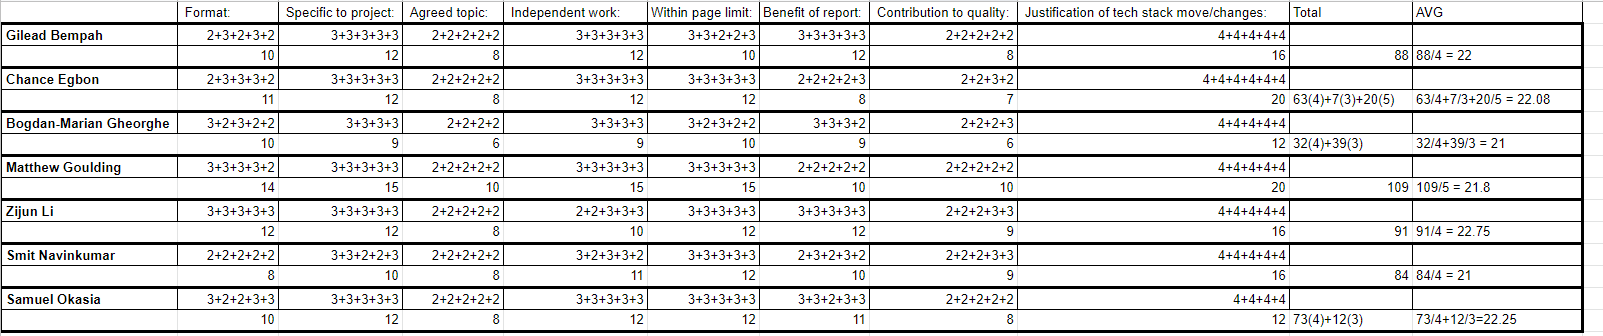
\includegraphics[width=1\textwidth]{./images/Comments.png}
	\label{Fig.Comments}
\end{figure}

\newpage

\section{\href{https://13.40.143.199/}{Walking skeleton/MVP}}

{\small

\subsection{Introduction}

Our project is a web-based application that helps with time management. It combines features of a scheduler and a to-do list, and also provides email notifications. With the anti-procrastination feature, you can control your own access to websites once you activate it. In addition, the application includes a timer and alarm to help you stay on track. The Diary feature allows you to add more details about upcoming events. The application also includes productivity analysis tools to help you track your progress and review your history.

\subsection{Scheduler}

In the Scheduler feature, the front-end and the database should work together to provide the users’ schedule. It should mainly consist of calendar-like features where the user can view their schedule for the day/week/month. It should also provide a view of the users’ current schedule, and the user should be able to interact with the scheduler to perform certain actions. Functions should allow the user to perform said actions, e.g clicking on a particular schedule for further details, editing a particular schedule, adding or removing a particular schedule, and the database should update accordingly when the user makes changes. 

API integration will be needed to allow the front-end and database to work together to display the users’ schedule, e.g the front-end sends a request to the database to get the data so it can be presented to the user. API integration is also needed to link the scheduler feature and the notification feature, as the notification feature notifies the user of their next schedule, and testing will be conducted to ensure that the scheduler works as intended (so it displays the correct schedule) and the user receives the notification for their next schedule on time.

Since the Scheduler displays the users’ schedule for the day/week/month as well as their current schedule, it needs to be linked to the current date and time so that it does not display the wrong schedule.

\subsection{To-do List}

The seamless synchronisation between the front-end and the database is the main focus of the Todo List MVP. To accomplish this, the TodoListItem object has been created with properties like heading and description (string types), creationTime and lastEditedTime (instance kinds), and finished (boolean type). Our technology stack uses Angular for front-end development and Spring Boot for back-end development, which allows for efficient communication between the two layers.

For the Todo List, important MVP characteristics include:

\begin{itemize}[itemsep=0.5\itemsep, parsep=0\parsep]
	\item Adding all finished things and to-dos.
	\item switching items with a single tap between the to-do and accomplished lists.
	\item showing thorough details when a to-do item is clicked.
	\item enabling the title and description of a to-do item to be updated by users within the details box.
\end{itemize}

We are integrating pertinent databases management frameworks and APIs to guarantee data permanence and uphold data integrity. We have also put security measures in place to safeguard user data and follow best practises.
Also, the front-end design needs to be simple and easy to use. As the project develops, this component will be further polished.
We use thorough testing and debugging techniques throughout the development process to ensure that the feature is stable and reliable before release. DevOps approaches help us to speed development and ensure that users receive new features and problem fixes more quickly.


\subsection{Anti-procrastination}

The current functionality of the Anti-Procrastination MVP is the ability to add blocked websites to the websites list; however, if the user adds the website as a timed blockage, there would be no option for that website block to be removed unless the timer expires. This functionality may be changed later as the user could input a large number in the day's number box on the page and cause them inconvenience.

A countdown timer has been included in the Dynamic List so that the user can see the time remaining until websites they have blocked get unblocked. The countdown timer decreases even  as the user closes the window.

The page's front-end design is adequate, but it may still be enhanced to make it more pleasant for users to use. It might also need to be adjusted to seem more in line with the other web pages and features that will be introduced to the programme.

Currently, the user can add more items to the blocked websites list and start a countdown timer, but these do not actually block the website itself so this is still a work in progress. The backend of this part looks fine, but it would be better to run more stress testing on it to find any bugs (3 found and fixed).
The Database is still a work-in-progress, but we anticipate implementing it shortly.

\subsection{Diary}

\subsubsection*{Diary MVP Current status}
Currently, the Diary MVP only stores the unfinished HTML file of the Diary feature. The MVP only holds the frontend of the Diary feature as no backend has been implemented yet. At this stage, HTML and CSS have been used to create the visual aspect of the navigation system of the Diary webpage. 

The navigation menu will be used by the user to navigate through the web application and make use of the various available features. Since not all the features have been fully developed the links are void and The page looks shallow because the page's main contents are still being developed. 

\subsubsection*{Diary MVP Goal status}
The final status of the Diary MVP should reflect the initial design that was submitted in the first Assignment. The MVP should hold the full stack of the Diary feature, this should include the backend and the frontend of the Diary webpage. 

The frontend should provide a way for the user to interact with the system and make use of the diary feature. It should allow the user to navigate through the web application, create and delete events by adding or deleting to the to-do list, write records related to items in the to-do list, and navigate through the scheduler to find and view other daily records. The feature’s interface should be well-detailed, all text should be easy to read and understand, all visible elements should be well-spaced, it should have a good color scheme and it should be similar to the initial design.  

The backend should provide a way to store, edit and delete information. It should help create a relationship between the Diary features and the scheduler and the to-do list feature. It should allow the user to indirectly make use of the database. When the add new event is clicked a new to-do list item should be created in the to-do table, when the delete event button is clicked a specific item should be deleted from the to-do table.

\subsection{Alarm/Timer}

The MVP so far has a basic user interface which is still in development in order to create an easy to use environment for the user. Currently it has the basic shape with the titles and a couple of buttons. It should allow the user to create alarms and timers seamlessly and everything should be self-explanatory on what it does. There will be a list of alarms and timers with each one having a button for pausing/playing and a button to delete the whole thing. There will be an add button to create a new alarm/timer which will then add one to the list, where its name and time can be initialised.
The backend implementation will start after there is a sufficient UI. For the Alarm/Timer the important MVP criteria include:
\begin{itemize}[itemsep=0.5\itemsep, parsep=0\parsep]
	\item Being able to create an alarm which will count down from a given time when started by the user.
	\item Being able to create a timer which will count up when started by the user.
	\item Being able to delete singular alarms/timers.
	\item Being able to clear every single alarm and timer.
\end{itemize}
The database implementation will follow after the backend is finished and it will store past alarms timers that have finished, which will allow them to be used again in the future. 

\subsection{History}
 
The MVP currently shows users where to input their test grades for specific subjects. It also allows them to visually see their overall test grades on a line graph so they are able to understand and see their progress. The MVP also has a section for users to see their upcoming test which include the subject name, date of test and their target for that test. The focus of the page is to provide users with a friendly interface where they can store their test grades and make analysis and their progress. The interface is designed to allow users to easily conclude if they are making progress or not. The current MVP does not compare the students actual progress to their target progress 

The backlend has not fully been developed and only has some basic functionality, it is yet to properly store and handle user data. The database has also not been developed but it is in its early stages of development, having the database will allow the back end to handle user data and feed it to the front end so it can visualise this data, hence the database is a key factor in this application and so is under development. 

\subsection{Email notifications}

Email Notification has been implemented, the application is now able to send template emails for verifying the account, password reset and also welcome email, new email templates such as DailyEmail, TaskDueSoon or WeeklyEmail are being developed, this was possible by modifying the application.yml and application-dev.yml and using SendGrid as our Email API and configuring jhipster to use SendGrid's SMTP configuration. 

The Notifications system will be linked with the scheduler and the To-Do List, it will send daily emails at a specific hour in the morning with tasks that need to be done that day and also with what has already been completed. The Notifications will be checking every day what is happening inside the to-do list and what tasks are not completed and then will get the needed information from the database to complete the DailyEmail template.

There is also a front-end for the inbox which is also being developed, this will allow the emails to be accesible without needing to switch to your actual email outside the application and will provide a way for the user to better interact with his notifications.

A notification button represented with a bell icon will be implemented as well which will allow a small notifications window to pop-up which will show a few of the tasks that are done, which are due soon etc.

So mainly the notifications will be split between the daily email which will be sent to the user everyday and real-time notifications that will be present in the notifications window represented by the bell button which will have some logic that will send a notification when there is less than 12 hours remanining until a deadline for one of the tasks or send notification when a task is overdue.

A weekly email notification will also be implemented which will work with the history charts feature, presenting the user with his progress in the past week in a template email in case he is not checking the feature inside the app, this will allow the user to track the progress and use our application more frequently.

As a summary, the API has been implemented so the application now able to send emails to the users, email templates are being worked on and backend that will work with the scheduler, to-do list and history and will trigger the emails to be sent needs to be implemented.

}

\newpage

\begin{tcolorbox}[colback=gray!20, sharp corners, boxrule=0pt, boxsep=0pt, left=5pt, right=5pt, top=5pt, bottom=5pt]
\section{GDPR policy \& DPIA form}

\subsection{Team23-22 GDPR Policy}

Team23-22 is committed to protecting and respecting your privacy. This GDPR Policy ("Policy") outlines our practices regarding the collection, use, storage, and protection of your personal data in accordance with the General Data Protection Regulation (GDPR).

\subsubsection*{1. Definitions}
"Personal Data" refers to any information relating to an identified or identifiable individual.

"Processing" refers to any operation or set of operations performed on personal data, including collection, storage, use, modification, or deletion.

"Data Subject" refers to the individual whose personal data is processed.

\subsubsection*{2. Data Collection}
We collect personal data that is necessary for the purpose of providing our Time Management web application ("Service"). This may include your name, email address, and any other relevant information related to your time management tasks, goals, or preferences. We collect personal data when you:

Create an account or use our Service.

Contact us for support or other inquiries.

\subsubsection*{3. Purpose of Data Processing}
We process your personal data for the following purposes:

To provide and maintain our Service.

To personalize and improve your experience with our Service.

To communicate with you regarding updates, promotions, or other relevant information.

To ensure the security and integrity of our Service.
\subsubsection*{4. Consent}
By using our Service, you consent to the collection and processing of your personal data in accordance with this Policy. We will obtain your explicit consent before collecting or processing any sensitive personal data or using your data for a purpose not specified in this Policy.

\subsubsection*{5. Data Minimization and Accuracy}
We collect and process only the personal data that is necessary for the purposes specified in this Policy. We take reasonable steps to ensure that the personal data we process is accurate, complete, and up-to-date.

\subsubsection*{6. Data Retention}
We retain your personal data for as long as necessary to fulfill the purposes for which it was collected, or as required by law. Upon the expiration of the retention period, your personal data will be securely deleted or anonymized.
\end{tcolorbox}

\newpage

\begin{tcolorbox}[colback=gray!20, sharp corners, boxrule=0pt, boxsep=0pt, left=5pt, right=5pt, top=5pt, bottom=5pt]
\subsubsection*{7. Data Security}
We implement appropriate technical and organizational measures to protect your personal data from unauthorized access, disclosure, alteration, or destruction. These measures include encryption, access controls, and secure data storage.

\subsubsection*{8. Data Subject Rights}
You have the right to:

\begin{itemize}
	\item Access your personal data and receive a copy of the data we process.
	\item Request rectification of inaccurate or incomplete personal data.
	\item Request erasure of your personal data, subject to certain conditions.
	\item Object to or restrict the processing of your personal data.
	\item Withdraw consent to the processing of your personal data at any time.
	\item Lodge a complaint with the relevant data protection authority.
\end{itemize}

\subsubsection*{9. Data Processors and International Transfers}
We may engage third-party data processors to process your personal data on our behalf. We ensure that these processors comply with GDPR requirements and have appropriate safeguards in place to protect your personal data.

Your personal data may be transferred and processed in countries outside the European Economic Area (EEA). We take appropriate measures to ensure that these transfers are compliant with GDPR and that your personal data remains protected.

\subsubsection*{10. Changes to this Policy}
We may update this Policy from time to time. We will notify you of any significant changes and will obtain your consent if required by law or if the changes involve the use of your personal data for a new purpose.

\subsubsection*{11. Contact Information}
If you have any questions or concerns about this Policy or our data processing practices, please contact us at:
Team23-22,
Birmingham

Emails:
\begin{itemize}[itemsep=0.5\itemsep, parsep=0\parsep]
	\item bxg125@bham.student.ac.uk
	\item cee010@bham.student.ac.uk
	\item gxb035@bham.student.ac.uk
	\item mxg183@bham.student.ac.uk
	\item sxo183@bham.student.ac.uk
	\item sxn197@bham.student.ac.uk
	\item zxl183@bham.student.ac.uk
\end{itemize}

Date of Last Revision: 3-14-2023
\end{tcolorbox}

\newpage
\begin{tcolorbox}[colback=gray!20, sharp corners, boxrule=0pt, boxsep=0pt, left=5pt, right=5pt, top=5pt, bottom=5pt]
\subsubsection*{12. Data Protection Officer}
If required by GDPR or applicable laws, we will appoint a Data Protection Officer (DPO) to oversee our data protection activities, monitor compliance with this Policy, and act as a point of contact for data subjects and regulatory authorities.

\subsubsection*{13. Data Breach Notification}
In the event of a personal data breach that poses a risk to your privacy, we will promptly notify you and the relevant data protection authority in accordance with GDPR requirements. We will also take appropriate measures to mitigate the impact of the breach and prevent its recurrence.

\subsubsection*{14. Privacy by Design}
We are committed to incorporating data protection principles and privacy measures into the design of our Service from the outset. We continually review and update our practices to ensure compliance with GDPR and to protect your personal data.

\subsubsection*{15. Children's Privacy}
Our Service is not intended for children under the age of 16. We do not knowingly collect personal data from children under 16. If we become aware that we have collected personal data from a child under 16, we will take appropriate steps to delete such data from our systems.

\subsubsection*{16. Third-Party Links}
Our Service may contain links to third-party websites or services that are not governed by this Policy. We are not responsible for the privacy practices or content of these third-party sites. We encourage you to review the privacy policies of any third-party websites or services you may visit.

By using our Time Management web application, you acknowledge and agree to the terms of this Policy.
\end{tcolorbox}

\newpage

\subsection{DPIA Form}
\begin{figure}[H]
	\centering
	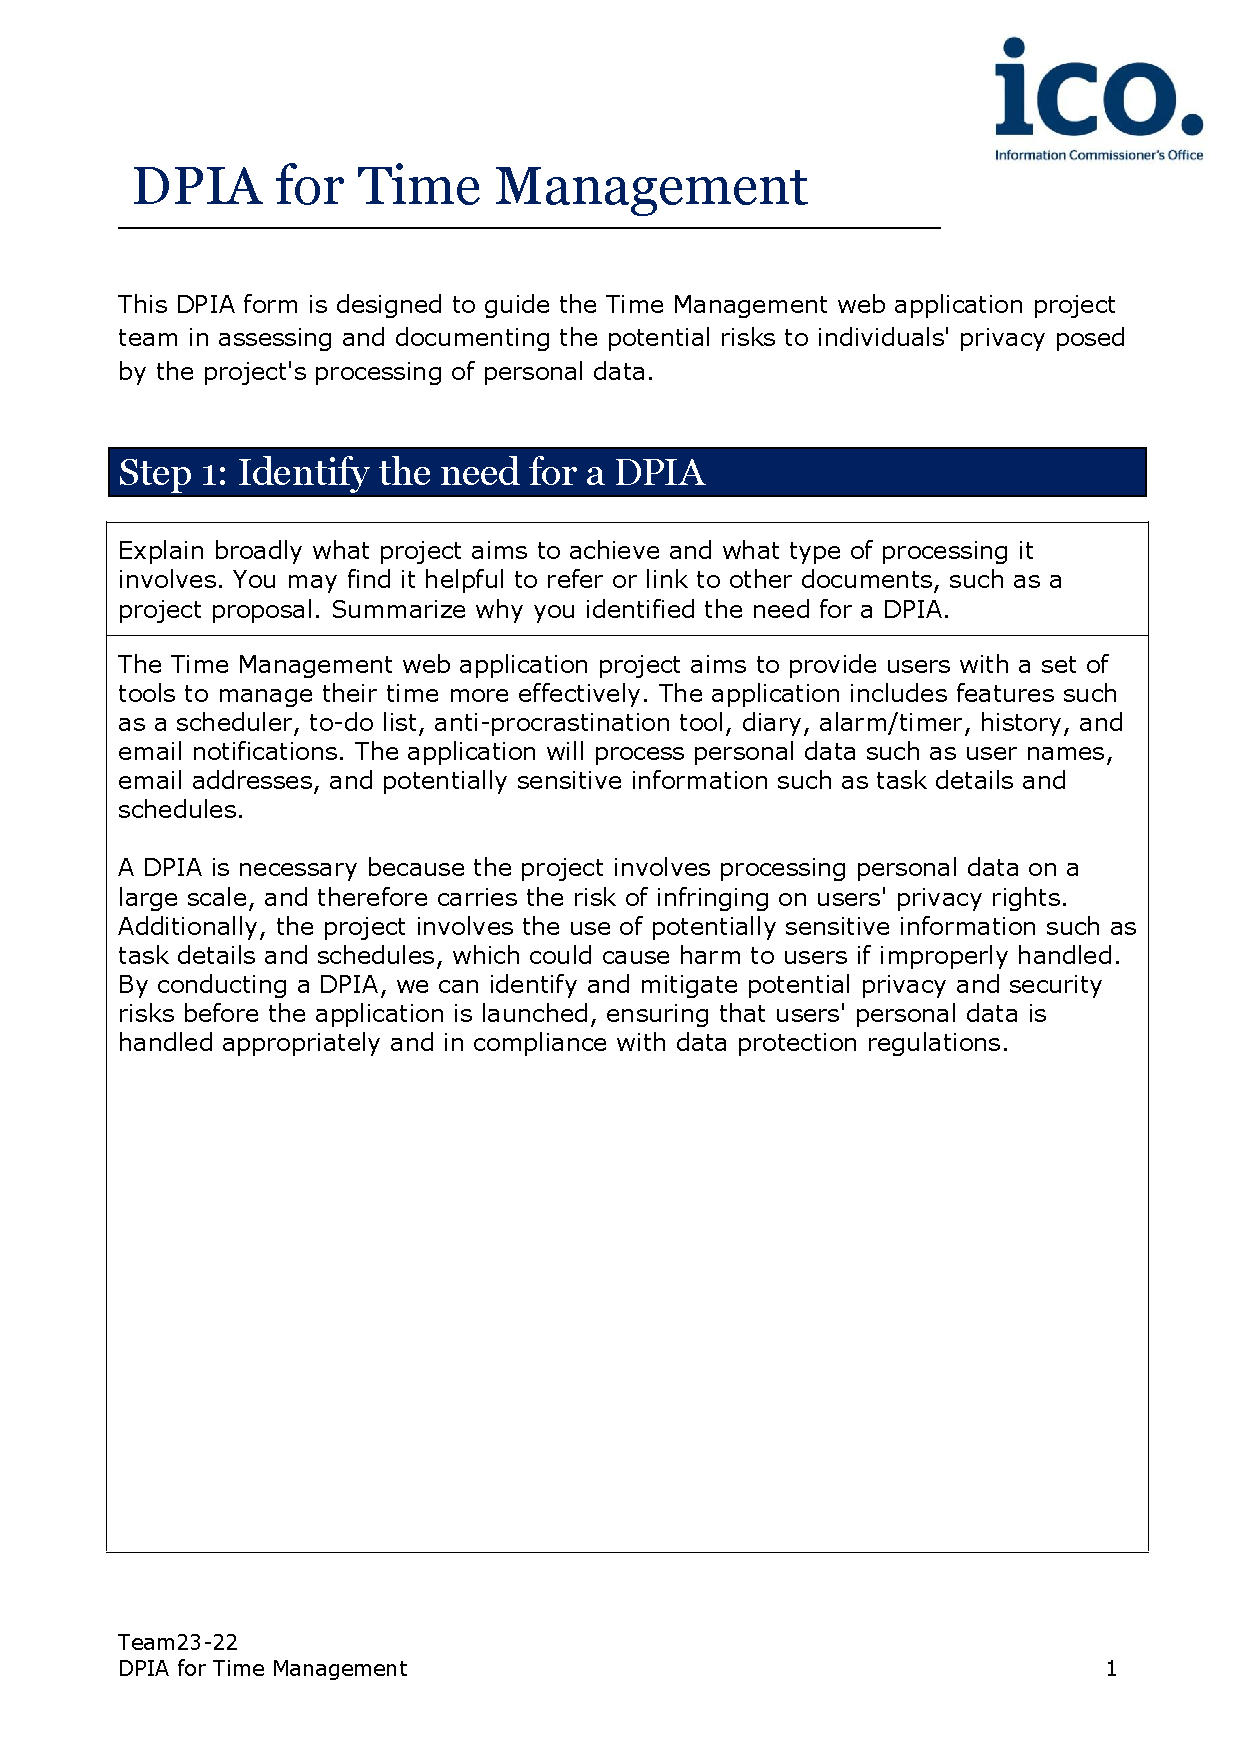
\includegraphics[width=1\textwidth]{./images/DPIA-Team23-22/DPIA-Team23-22_1.pdf}
	\label{Fig.DPIA_1}
\end{figure}

\begin{figure}[H]
	\centering
	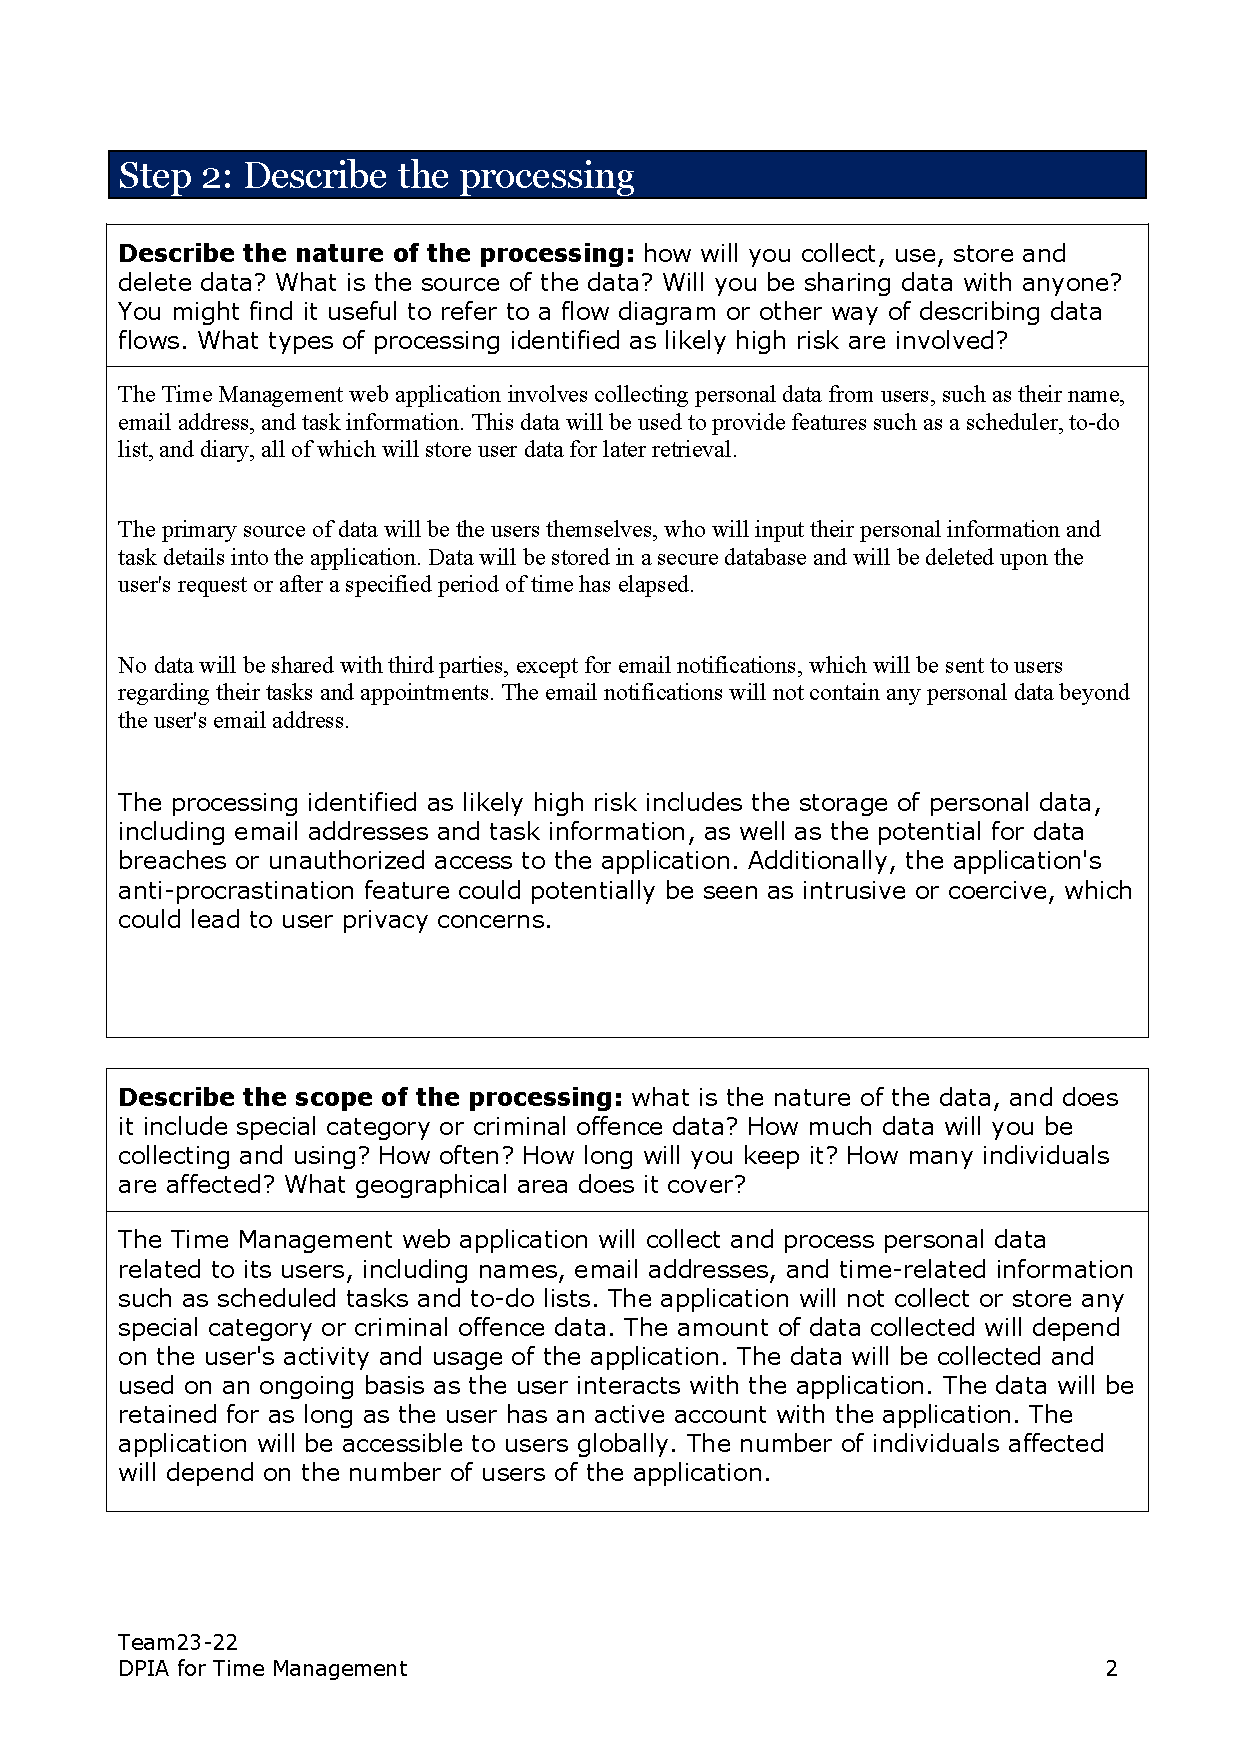
\includegraphics[width=1\textwidth]{./images/DPIA-Team23-22/DPIA-Team23-22_2.pdf}
	\label{Fig.DPIA_2}
\end{figure}
\begin{figure}[H]
	\centering
	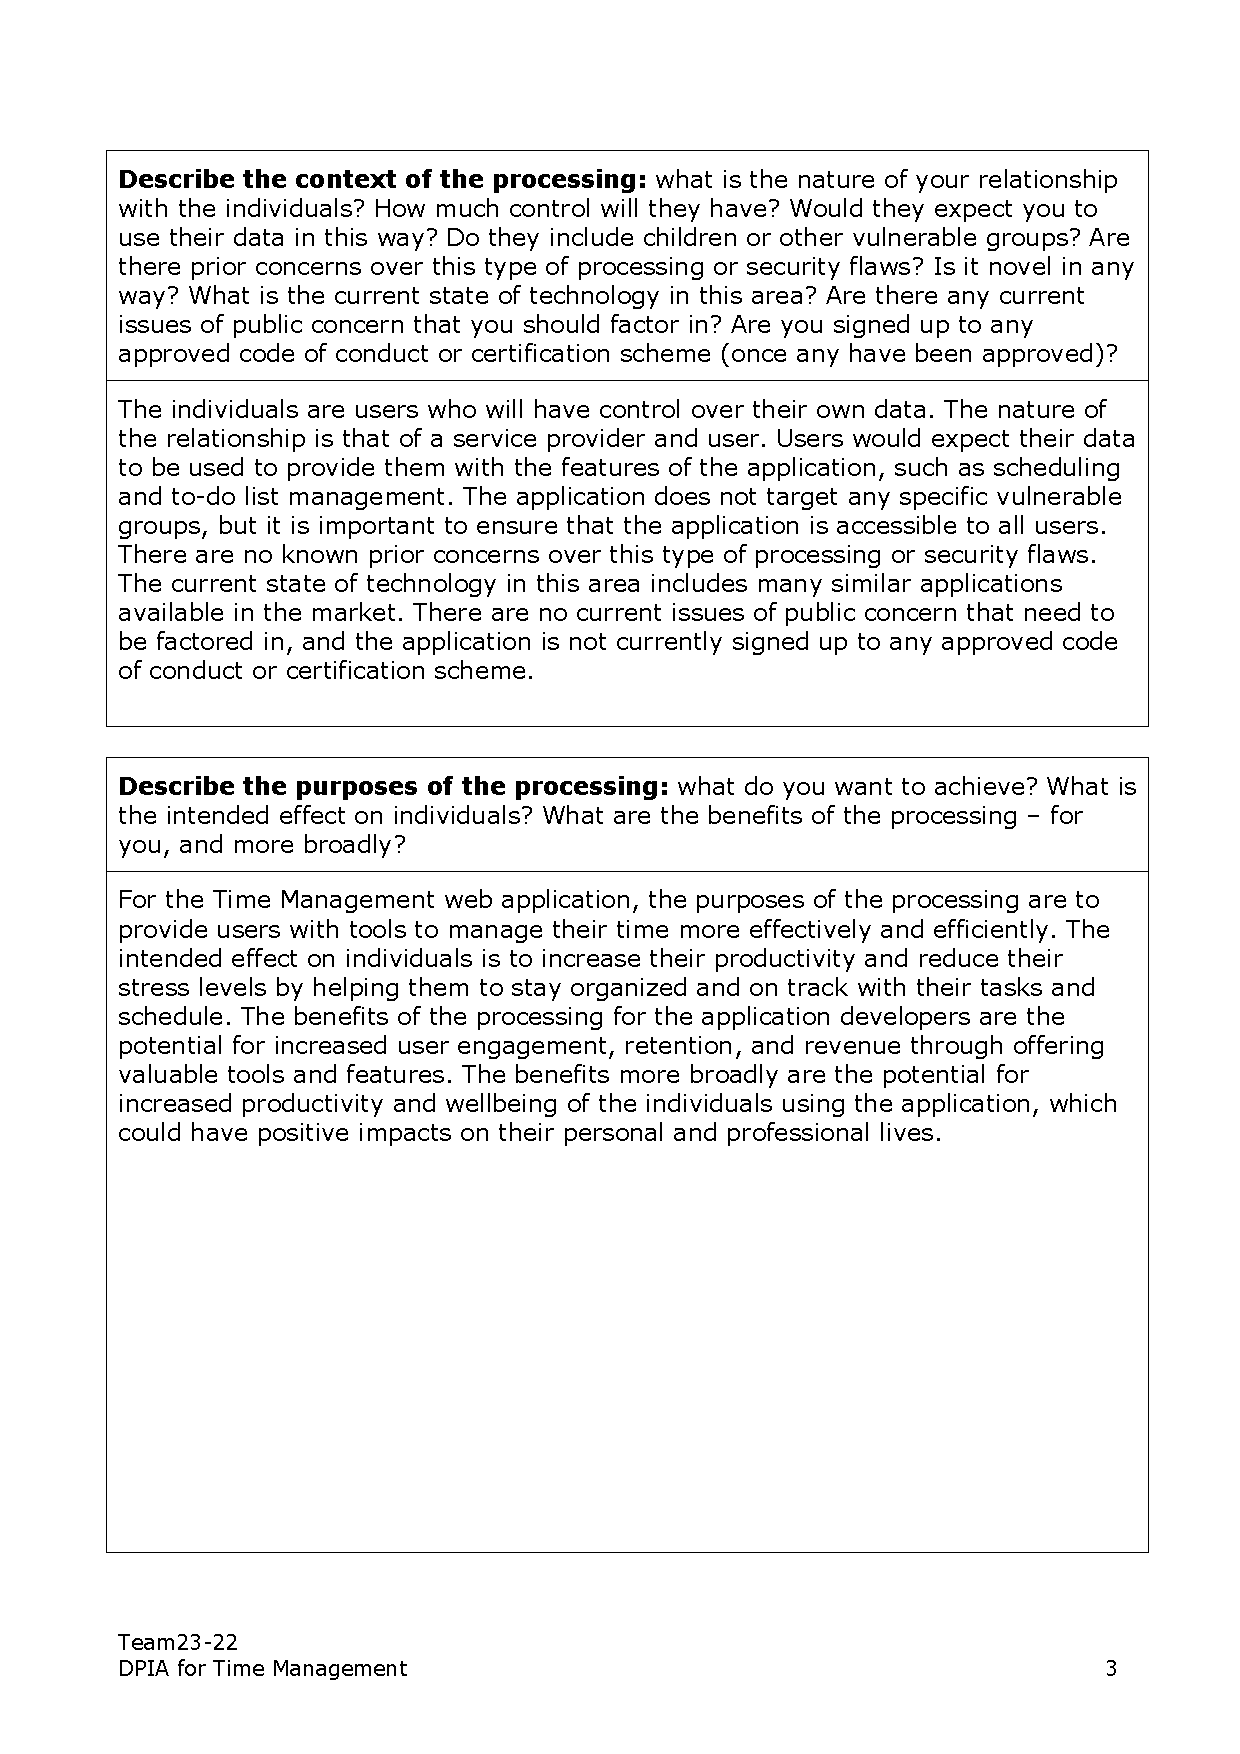
\includegraphics[width=1\textwidth]{./images/DPIA-Team23-22/DPIA-Team23-22_3.pdf}
	\label{Fig.DPIA_3}
\end{figure}
\begin{figure}[H]
	\centering
	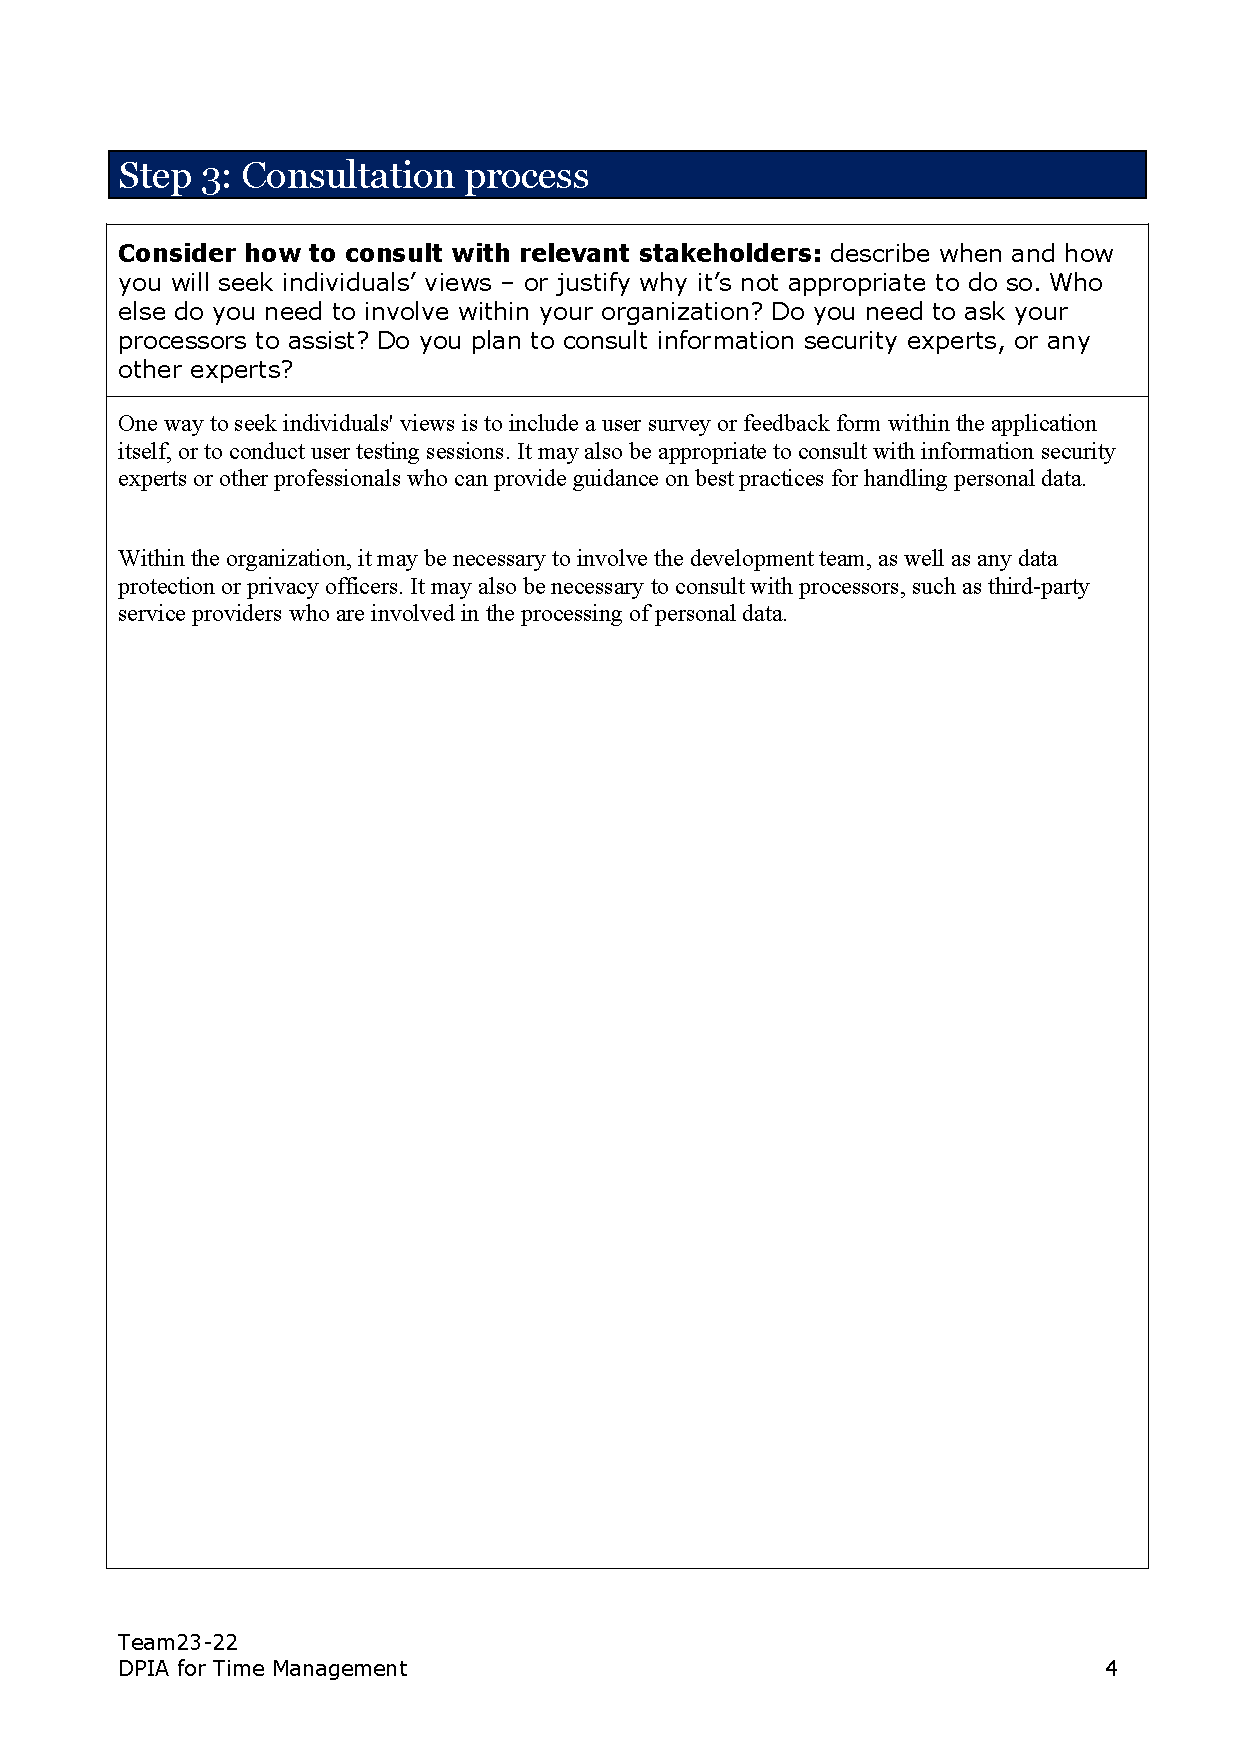
\includegraphics[width=1\textwidth]{./images/DPIA-Team23-22/DPIA-Team23-22_4.pdf}
	\label{Fig.DPIA_4}
\end{figure}
\begin{figure}[H]
	\centering
	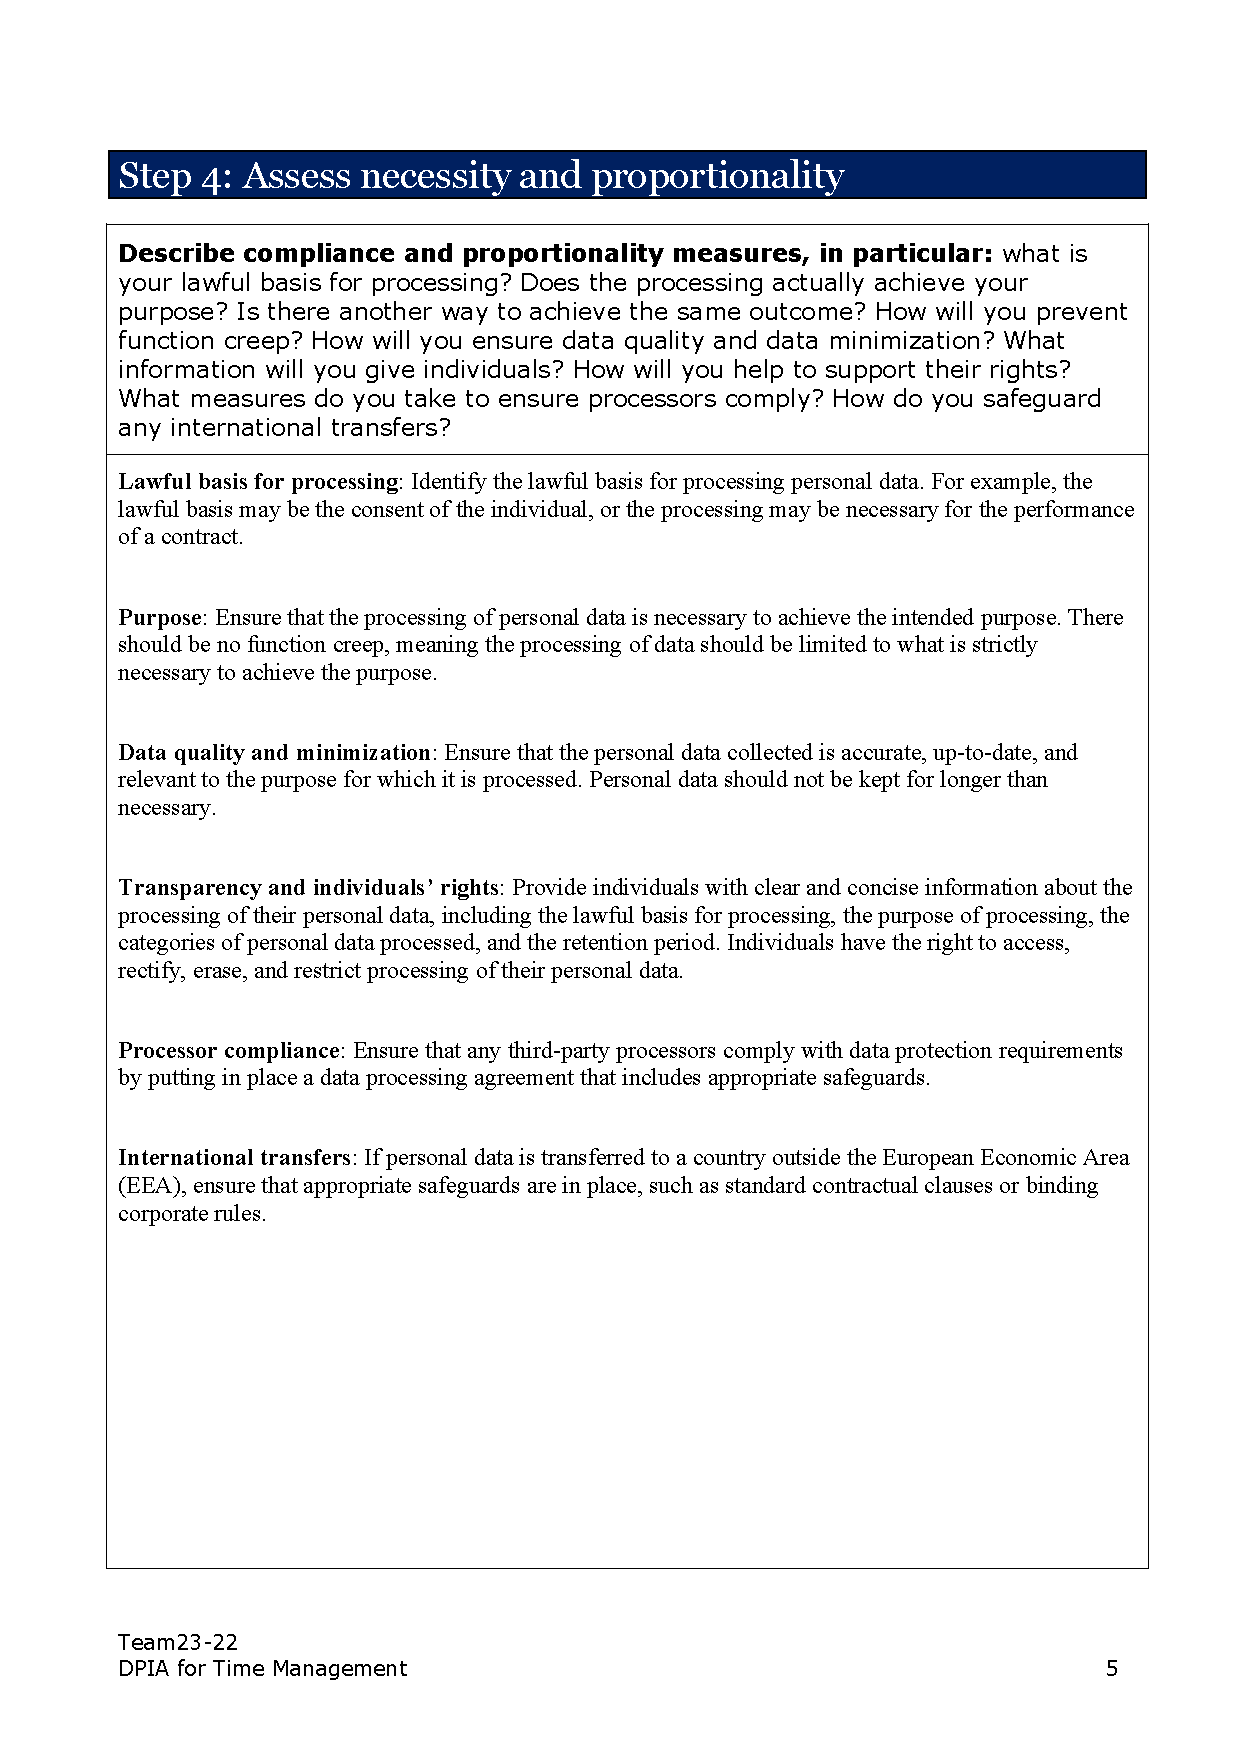
\includegraphics[width=1\textwidth]{./images/DPIA-Team23-22/DPIA-Team23-22_5.pdf}
	\label{Fig.DPIA_5}
\end{figure}
\begin{figure}[H]
	\centering
	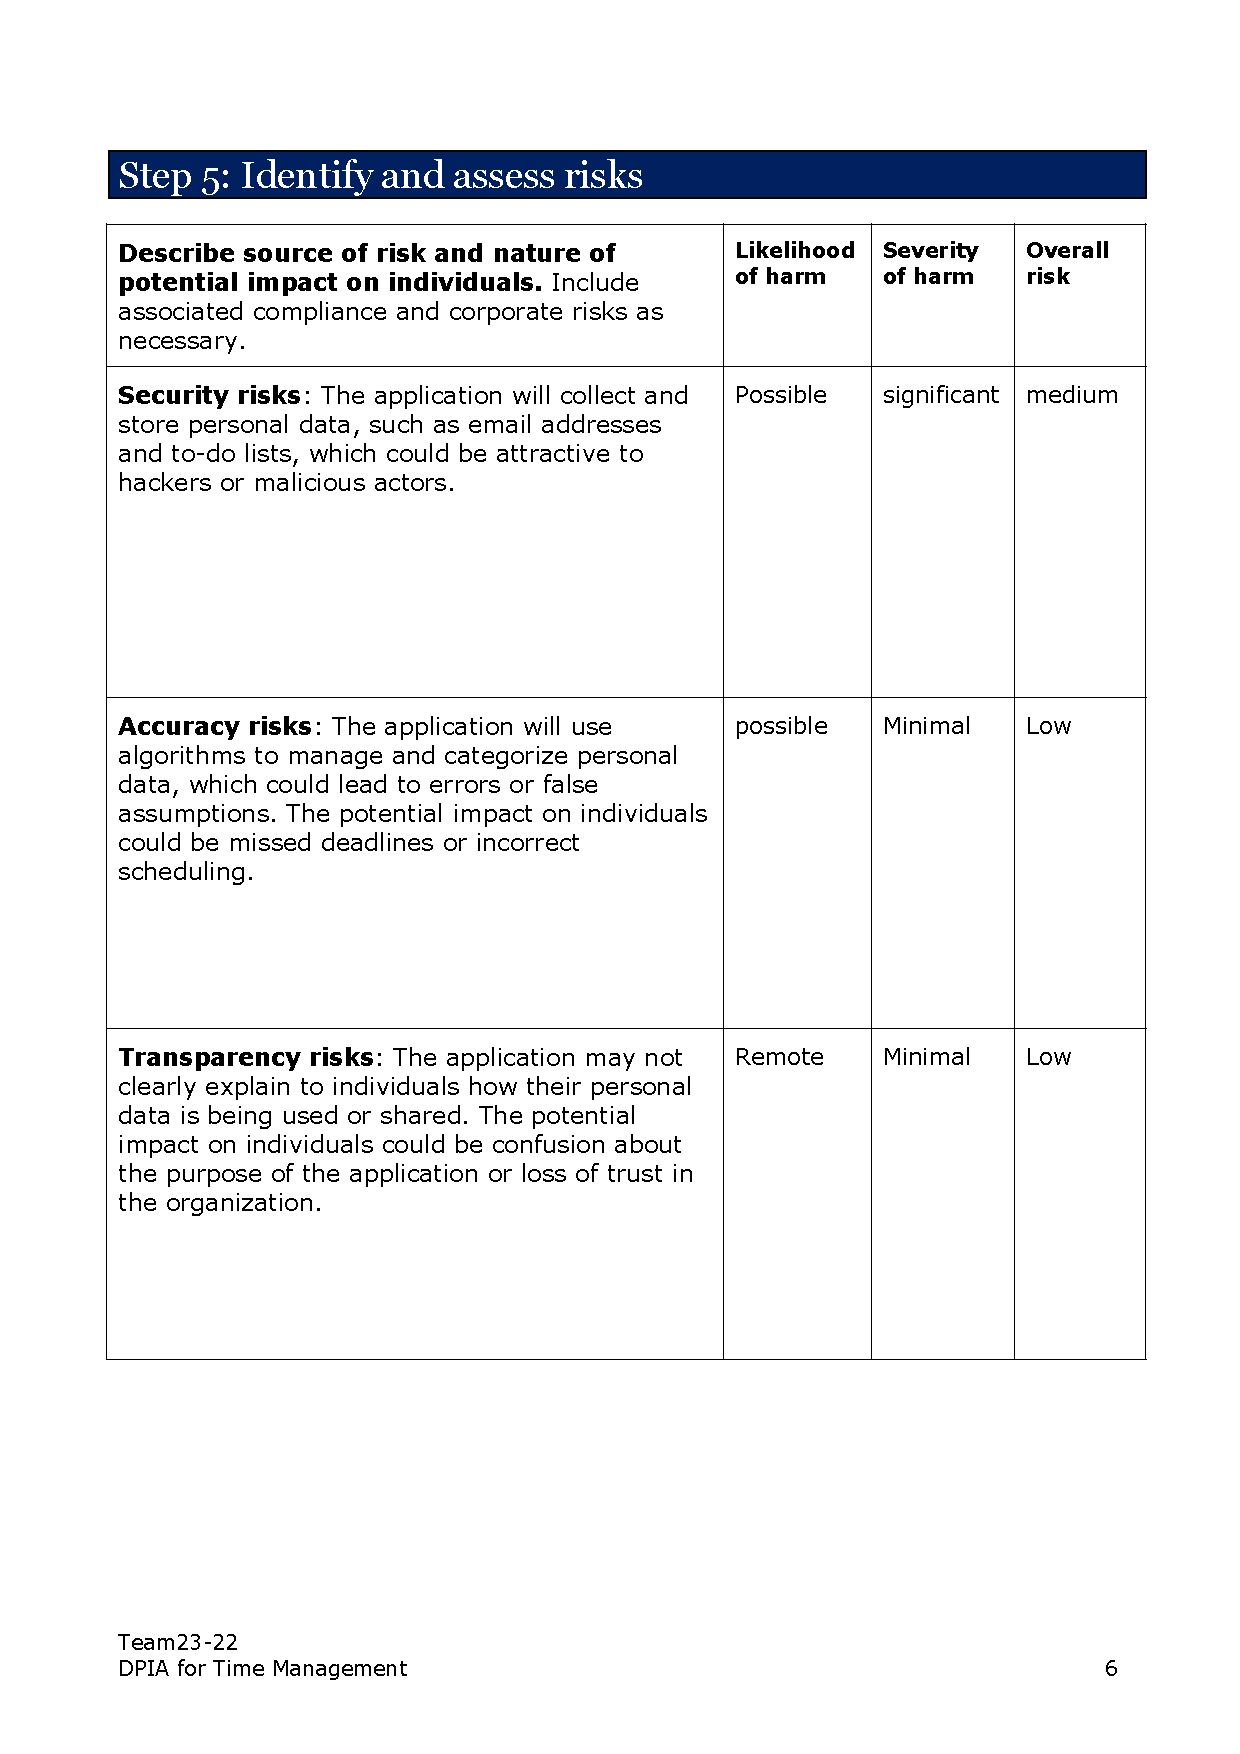
\includegraphics[width=1\textwidth]{./images/DPIA-Team23-22/DPIA-Team23-22_6.pdf}
	\label{Fig.DPIA_6}
\end{figure}
\begin{figure}[H]
	\centering
	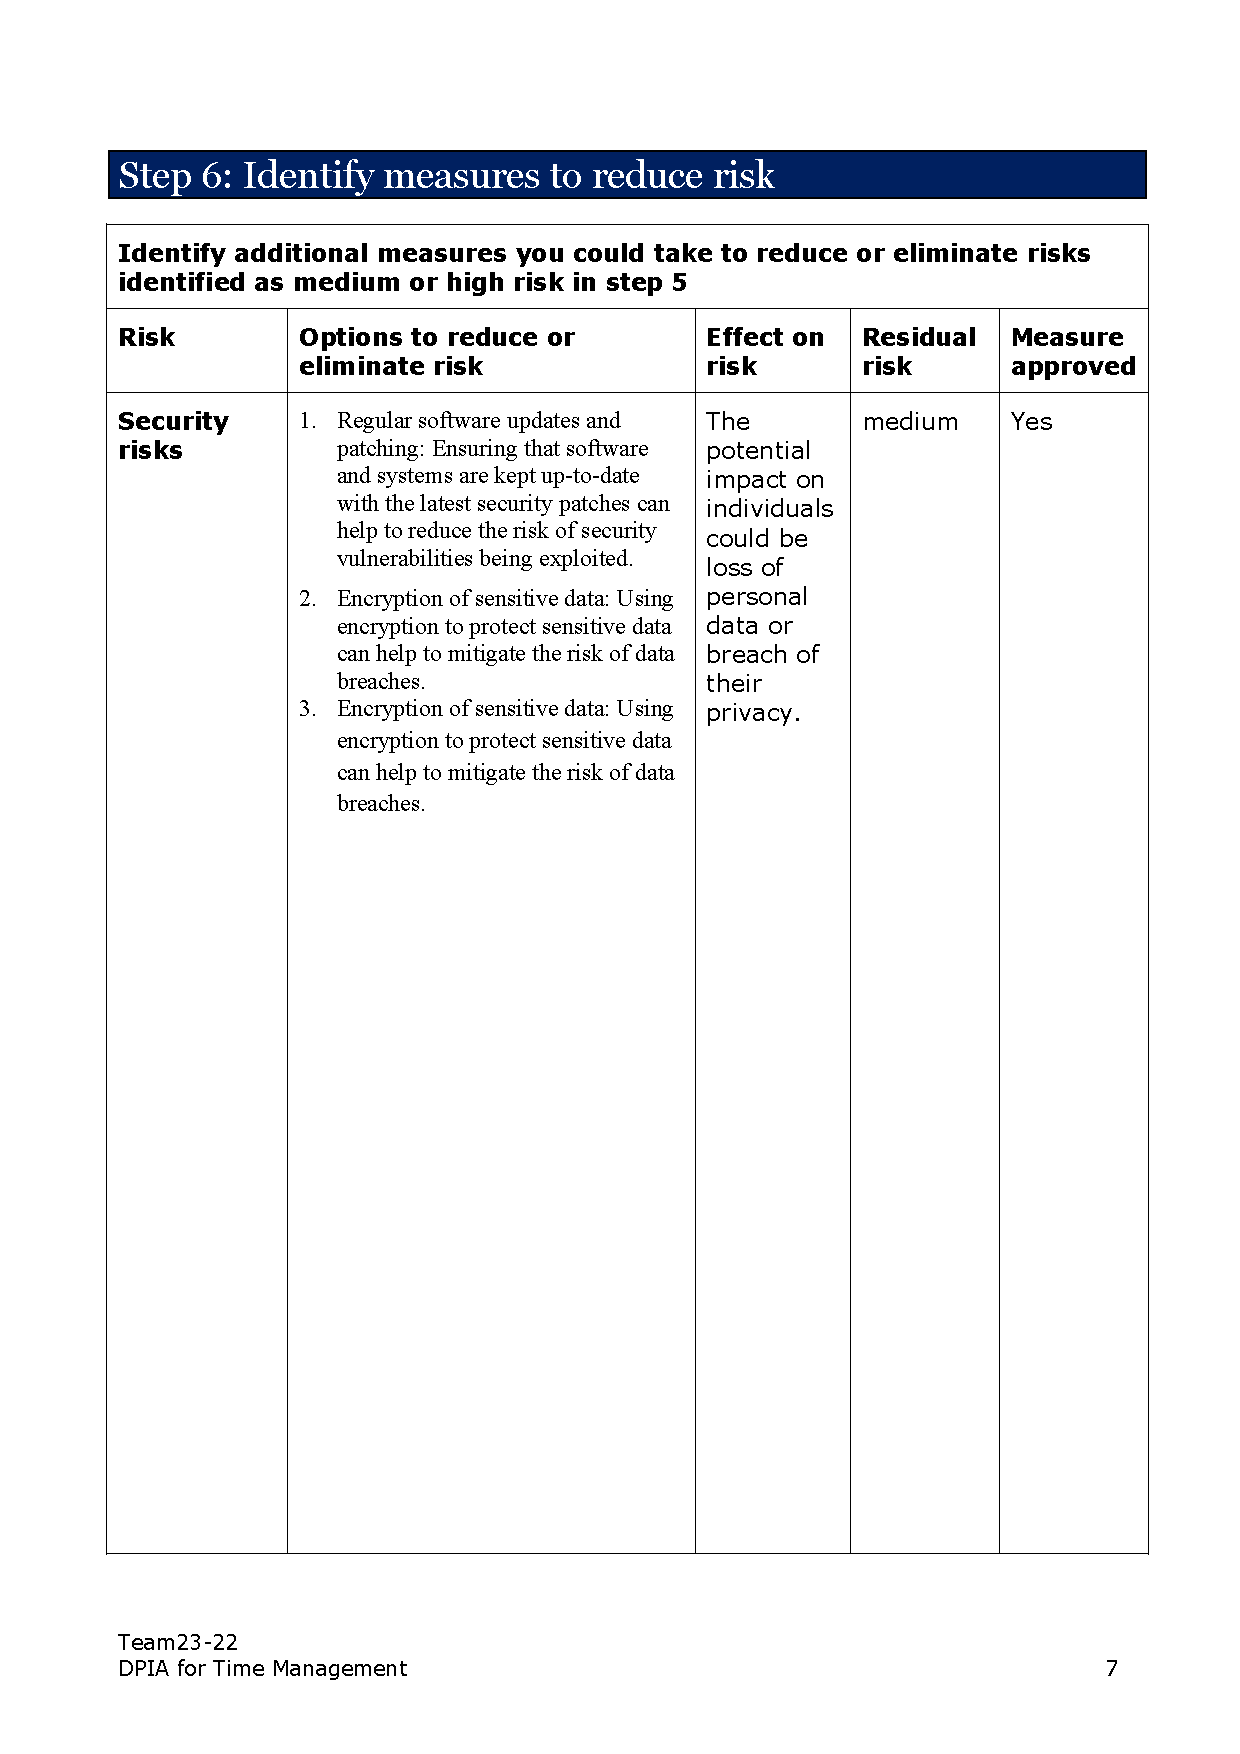
\includegraphics[width=1\textwidth]{./images/DPIA-Team23-22/DPIA-Team23-22_7.pdf}
	\label{Fig.DPIA_7}
\end{figure}

\section{Meeting diary}

{\noindent\begin{tabular}{|p{0.2\linewidth}|p{0.75\linewidth}|} 
	\hline
 \multicolumn{2}{|l|}{\textbf{Week 5: Meeting 1}}\\
 \hline
 \textbf{Date} & 28-2-2023\\
 \hline
 \textbf{Time} & 14:20-14:40(UK Time Zone)\\
 \hline
 \textbf{Venue} & LG23 (Seminar Room) in the Lower Ground Floor/Team Calls\\
 \hline
 \multirow{2}*{\textbf{Attendees}} & Meeting Chair: Christian Vergara Marcillo\\
 ~ & Other Participants: Chance Egbon, Matthew Goulding, Zijun Li, Samuel Okasia, Smit Navinkumar\\
 \hline
 \multirow{3}*{\textbf{Discussions}} & - we talked about how to allocate different topics of the tech stack to each team member. We also discussed the requirements for the tech report and how to ensure that all necessary information is included.\\
 ~ & - We had a discussion on the concept of Minimum Viable Product (MVP) and how it can be developed. We talked about the key features that should be included in an MVP and the steps required to create a successful MVP.\\
 ~ & -  we discussed with the TA on the recommended format for estimating the time required to complete different features. \\
 \hline
 \multirow{3}*{\textbf{Decisions Made}} & - Each member was assigned a topic related to the tech stack, and we need to create a corresponding tech report.\\
 ~ & - We agreed to use MVP/Skull walking in the project to develop a minimum viable product and iterate on it until it meets the desired level of functionality.\\
 ~ & - We decided we might use a Gantt chart to estimate time for feature cards and manage the project schedule and our estimation time should be similar to each others.\\
 \hline
\end{tabular}}

\newpage

{\noindent\begin{tabular}{|p{0.2\linewidth}|p{0.75\linewidth}|} 
	\hline
 \multicolumn{2}{|l|}{\textbf{Week 6: Meeting 1}}\\
 \hline
 \textbf{Date} & 7-3-2023\\
 \hline
 \textbf{Time} & 14:20-14:40(UK Time Zone)\\
 \hline
 \textbf{Venue} & LG23 (Seminar Room) in the Lower Ground Floor/Team Calls\\
 \hline
 \multirow{2}*{\textbf{Attendees}} & Meeting Chair: Christian Vergara Marcillo\\
 ~ & Other Participants: Chance Egbon, Gilead Bempah, Matthew Goulding, Zijun Li, Bogdan-Marian Gheorghe, Samuel Okasia, Smit Navinkumar\\
 \hline
 {\textbf{Discussions}} & The material on the Canvas website was rather ambiguous, so we asked the TA for further details on the S2 and what we needed to submit for it. He then took us through it. The one page technical report should be discussed among us as we divide the different parts among us, warning us to make sure none of us is doing the same part. The evidence of pipeline commit being us showing we pushed our own branches to the Gitlab is also proof that we have started developing, he said. He instructed us that the time estimation of the features should have a rough estimate in hours and a short description to justify the choice of time spent.\\
 \hline
 {\textbf{Decisions Made}} & Later, after speaking with one another on Discord, we made the decision to place all of the time estimates for our features in Google Spreadsheets and to get in touch with one another if we needed any more assistance with our assignments.\\
 \hline
\end{tabular}}

\hspace*{\fill}\\

{\noindent\begin{tabular}{|p{0.2\linewidth}|p{0.75\linewidth}|} 
	\hline
 \multicolumn{2}{|l|}{\textbf{Week 6: Meeting 2}}\\
 \hline
 \textbf{Date} & 8-3-2023\\
 \hline
 \textbf{Time} & 14:20-14:40(UK Time Zone)\\
 \hline
 \textbf{Venue} & Discord\\
 \hline
 {\textbf{Attendees}} & Gilead Bempah, Smit Navimkumar, Samuel Okasia \\
 \hline
 \textbf{Discussions} & We addressed the team project and the abilities we would need to acquire to see it through at this brief discussion.\\
 \hline
\end{tabular}}

\newpage

{\noindent\begin{tabular}{|p{0.2\linewidth}|p{0.75\linewidth}|} 
	\hline
 \multicolumn{2}{|l|}{\textbf{Week 7: Meeting 1}}\\
 \hline
 \textbf{Date} & 14-3-2023\\
 \hline
 \textbf{Time} & 14:20-14:40(UK Time Zone)\\
 \hline
 \textbf{Venue} & LG23 (Seminar Room) in the Lower Ground Floor/Discord Calls\\
 \hline
 \multirow{2}*{\textbf{Attendees}} & Meeting Chair: Christian Vergara Marcillo \\
 ~ & Other Participants: Chance Egbon, Gilead Bempah, Bogdan-Marian Gheorghe, Matthew Goulding, Zijun Li, Samuel Okasia\\
 \hline
 \multirow{4}*{\textbf{Discussions}} & TWe asked the TA for clarification on the M2 Submission, and he said that the S3 task allocation Feature cards that we need to submit need to have some description attached to them, and we should decide how to assign them among ourselves. The TA looked at our progress with our Jhipster application and gave us feedback. He also advised us that if we were struggling in any parts of our projects or having any issues with it, we should go to the lab sessions for any assistance.\\
 ~ & He advised us that in order for our website to comply with the standards provided to us, the GDPR and DPIA forms should be displayed anywhere on it.\\
 ~ & He gave us a thorough explanation of the format of the MVP report, saying that even if it isn't finished, it should at least demonstrate some functionality, and that to get the best grades for MVP report, it should demonstrate some front-end, back-end, and database capability.\\
 ~ & He reminded us that this was a team project and that we should be cooperating to complete it before the meeting came to a conclusion.\\
 \hline
 \multirow{2}*{\textbf{Decisions Made}} & The MVP report we would create would be divided into five primary sections, each with distinct specifications.\\
 ~ &Each Kanban board will have a description written for the S3 allocation, and the jobs will be divided between us.\\
 \hline
\end{tabular}}

\section{S3 task allocation \& planning}

\subsection{Gilead Bempah}

\begin{figure}[H]
	\centering
	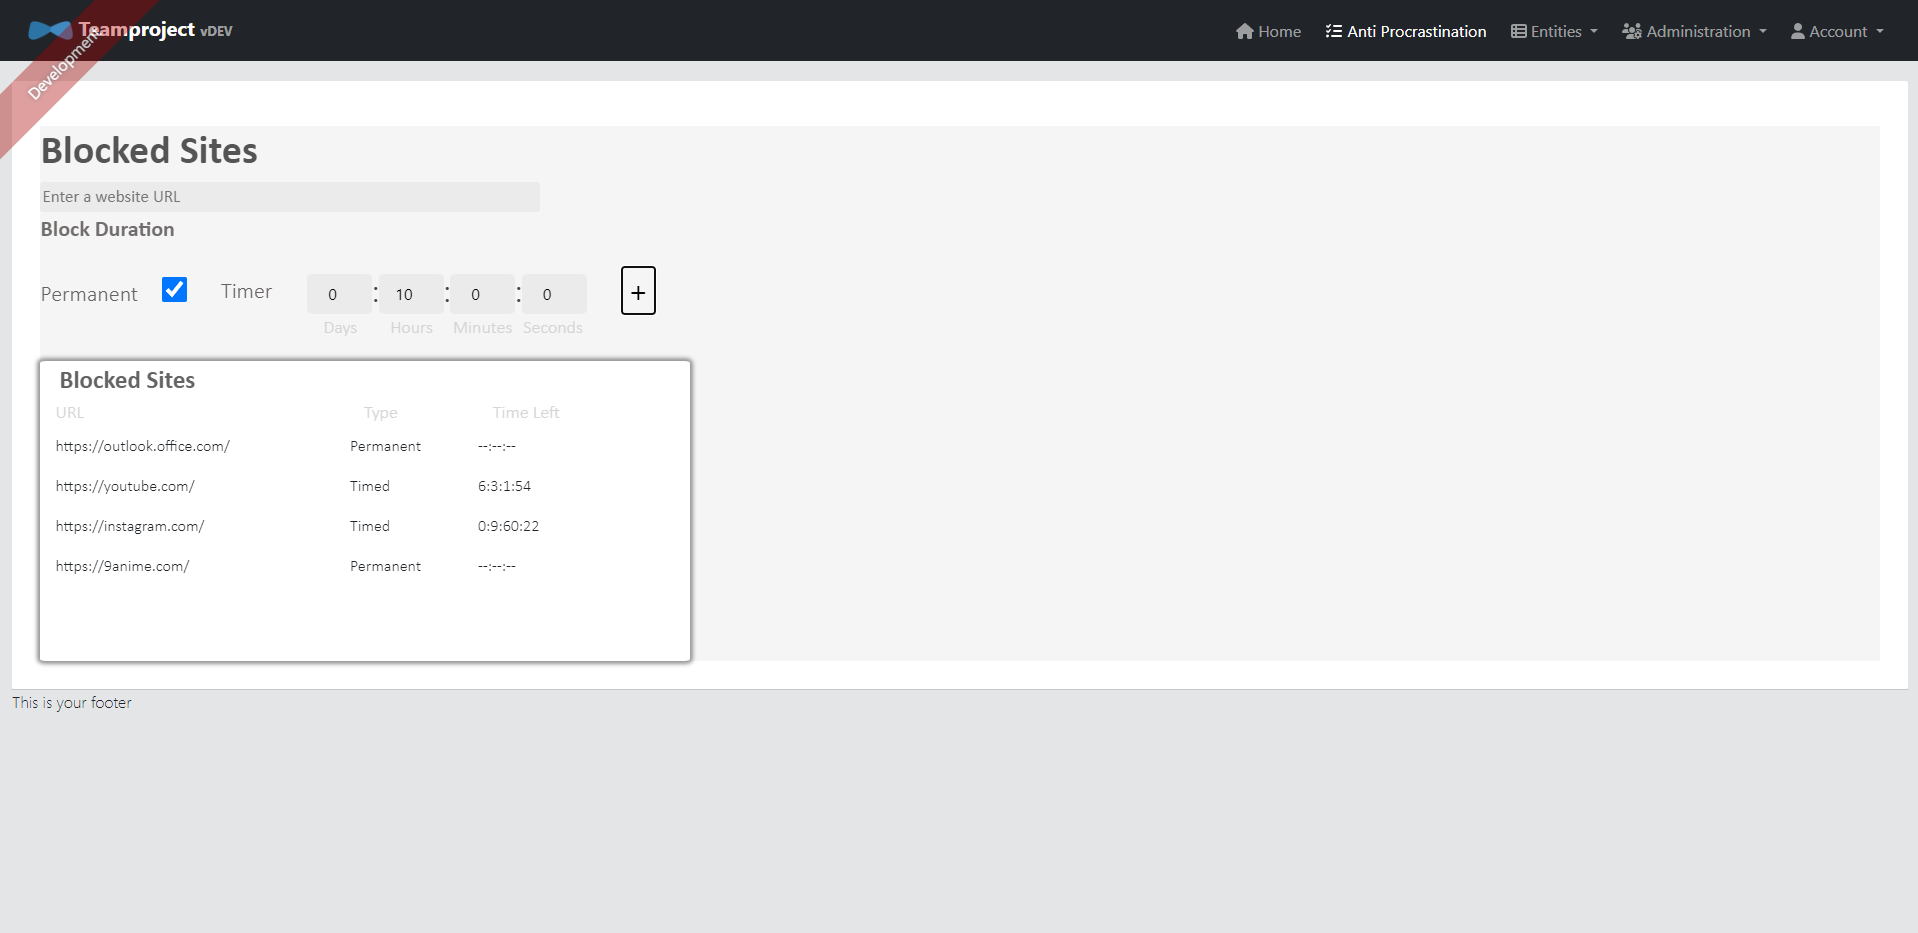
\includegraphics[width=1\textwidth]{./images/Anti.png}
	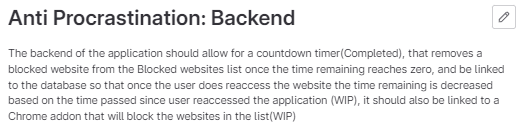
\includegraphics[width=1\textwidth]{./images/Anti_Backend.png}
	
\includegraphics[width=1\textwidth]{./images/Anti_Block_site.png}
	
\includegraphics[width=1\textwidth]{./images/Anti_Interface.png}
	\caption*{Anti Procrastination: Gilead Bempah}
	\label{Fig.Anti_Procrastination}
\end{figure}

\subsection{Zijun Li}

\begin{figure}[H]
	\centering
	
\includegraphics[width=1\textwidth]{./images/Todo_List.png}
	
\includegraphics[width=1\textwidth]{./images/Todo_List_Details.png}
	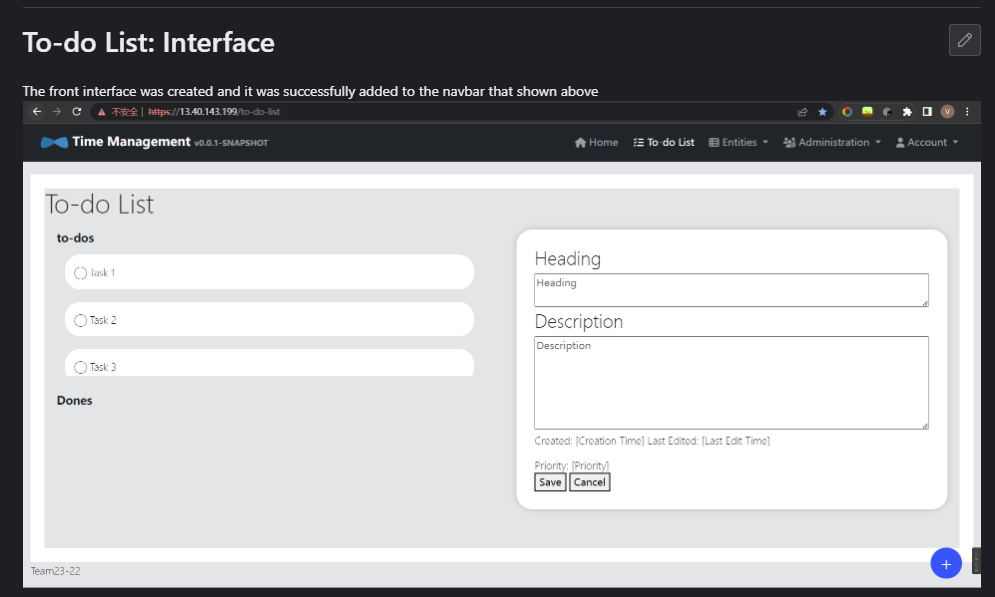
\includegraphics[width=1\textwidth]{./images/Todo_List_Interface.png}
	
\includegraphics[width=1\textwidth]{./images/Todo_List_Done_Item.png}
	
\includegraphics[width=1\textwidth]{./images/Todo_List_Todo_Item.png}
	\caption*{Todo List: Zijun Li}
	\label{Fig.Todo List}
\end{figure}

\subsection{Smit Navimkumar}

\begin{figure}[H]
	\centering
	
\includegraphics[width=1\textwidth]{./images/Scheduler.png}
	
\includegraphics[width=1\textwidth]{./images/Scheduler_Database.png}
	
\includegraphics[width=1\textwidth]{./images/Scheduler_Interface.png}
	
\includegraphics[width=1\textwidth]{./images/Scheduler_Live.png}
	\caption*{Scheduler: Smit Navimkumar}
	\label{Fig.Scheduler}
\end{figure}

\subsection{Chance Egbon}

\begin{figure}[H]
	\centering
	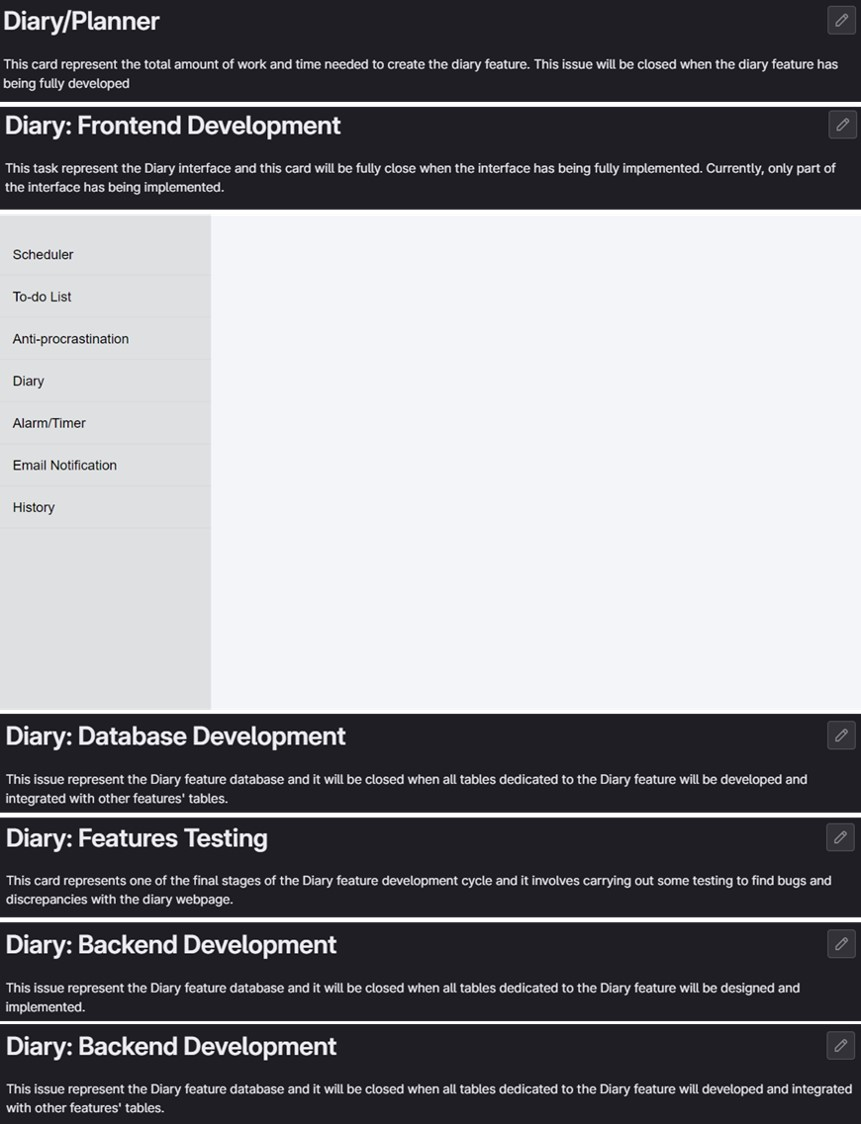
\includegraphics[width=1\textwidth]{./images/Diary.jpg}
	\caption*{Diary: Chance Egbon}
	\label{Fig.Diary}
\end{figure}

\subsection{Matthew Goulding}

\begin{figure}[H]
	\centering
	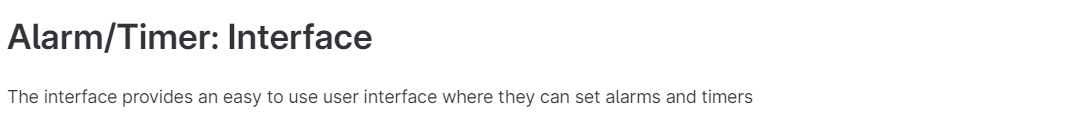
\includegraphics[width=0.8\textwidth]{./images/Alarm_Interface.png}
	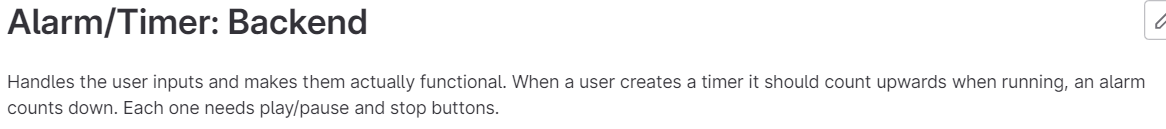
\includegraphics[width=0.8\textwidth]{./images/Alarm_Backend.png}
	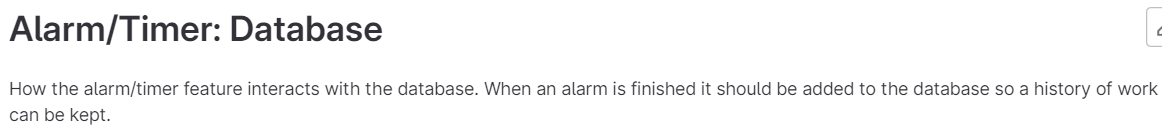
\includegraphics[width=0.8\textwidth]{./images/Alarm_Database.png}
	\caption*{Alarm/Timer: Matthew Goulding}
	\label{Fig.Alarm}
\end{figure}

\subsection{Samuel Okasia}
 
\begin{figure}[H]
	\centering
	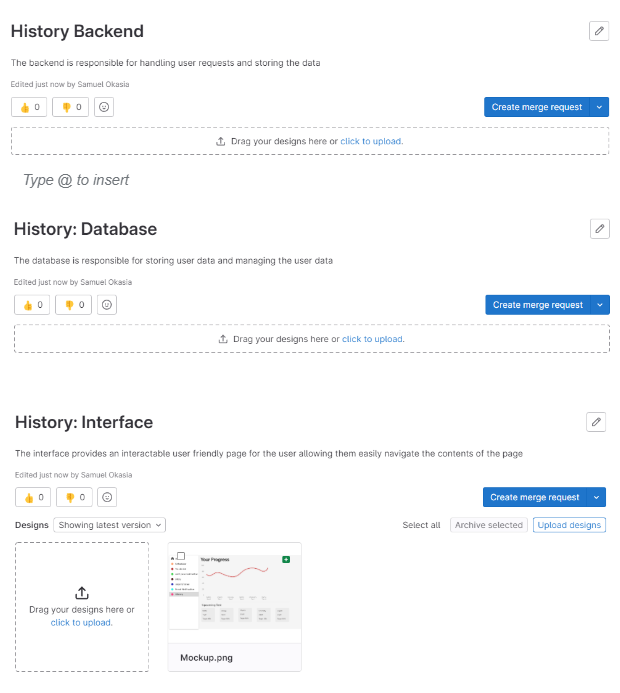
\includegraphics[width=0.8\textwidth]{./images/History.png}
	\caption*{History: Samuel Okasia}
	\label{Fig.History}
\end{figure}

\subsection{Bogdan-Marian Gheorghe}

\begin{figure}[H]
	\centering
	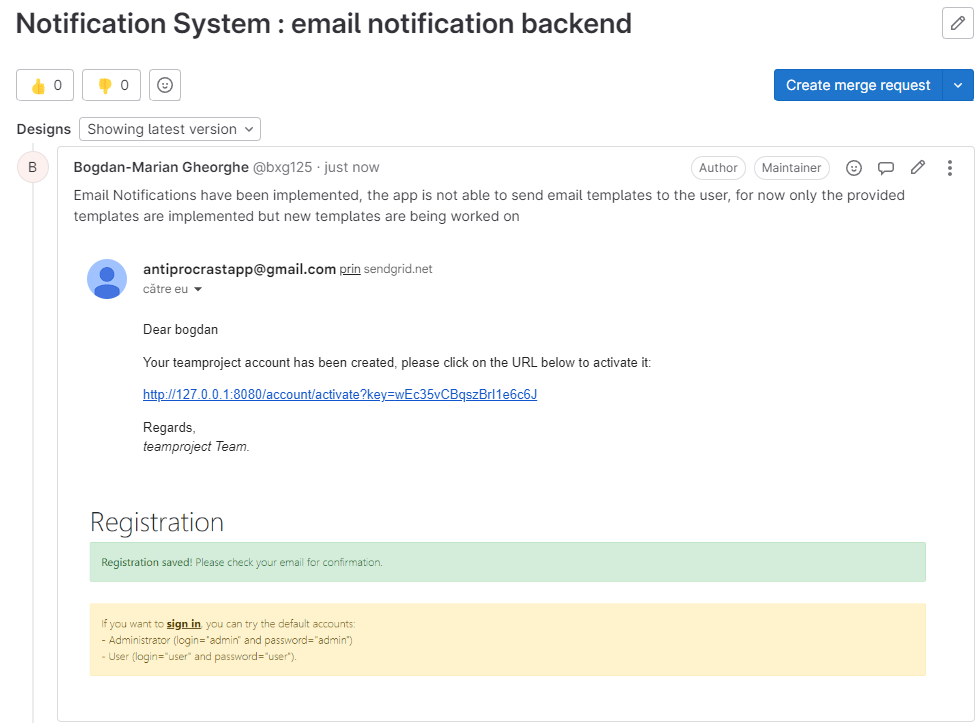
\includegraphics[width=0.75\textwidth]{./images/Email_backend.png}
	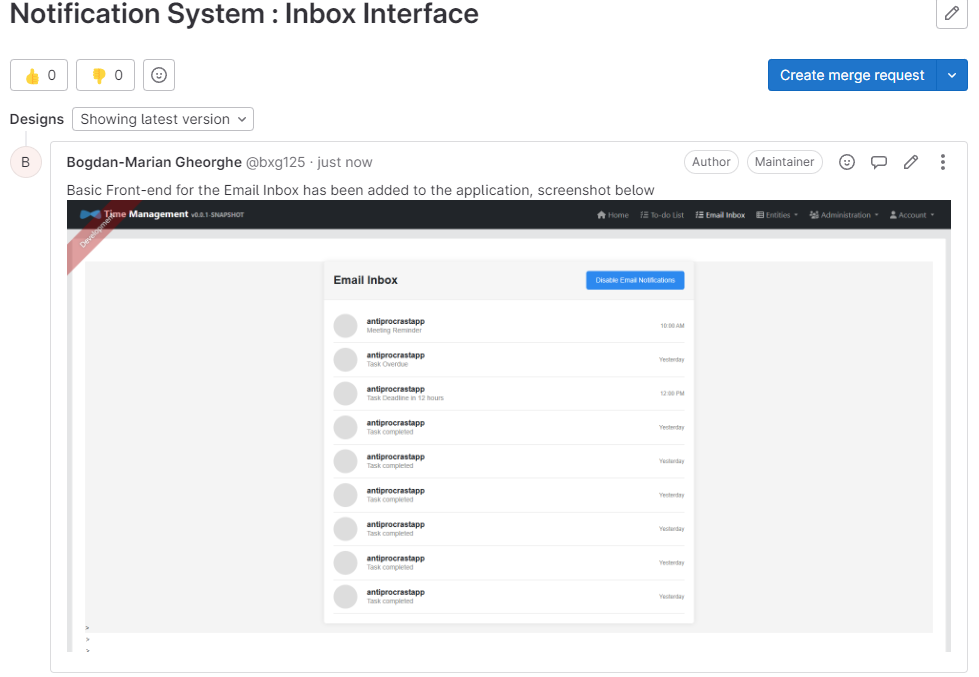
\includegraphics[width=0.75\textwidth]{./images/Email_Inbox_Interface.png}
	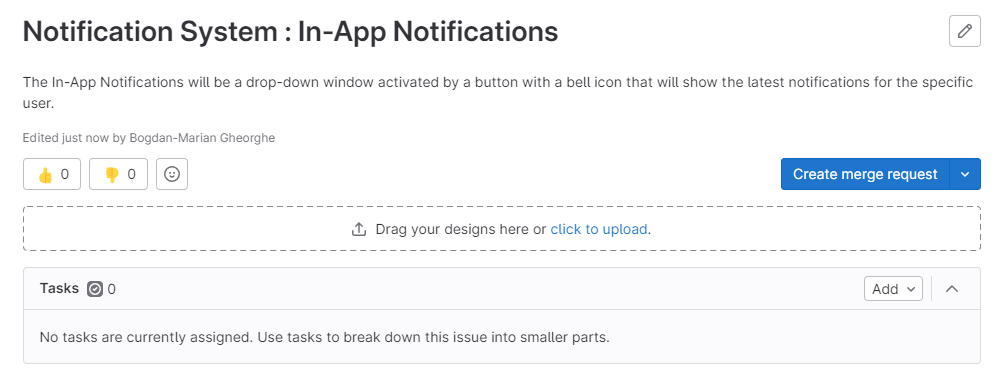
\includegraphics[width=0.75\textwidth]{./images/Email_Inapp.png}
	\caption*{Email Notification: Bogdan-Marian Gheorghe }
	\label{Fig.Email}
\end{figure}

\end{document}